Un lac qui alimente une région en électricité voit son niveau d'eau baisser depuis le début des années 2000.

	En 2020, le niveau du lac était d'environ \np{1100} mètres au-dessus du niveau de la mer.

	En dessous de \np{1020} mètres, le niveau du lac est insuffisant pour permettre la production d'énergie hydroélectrique.

	\subsection*{Partie A -- Étude d'un modèle discret}

	Dans cette partie, on estime que le niveau du lac, mesuré au-dessus du niveau de la mer, baisse de 1\,\% tous les ans.

	On définit la suite $(u_n)$ telle que $u_n$ représente le niveau du lac en mètres $n$ années après 2020, c'est-à-dire en $2020+n$.

	\begin{minipage}{0.7\linewidth}
		On a alors $u_0 = \np{1100}$.

	\begin{enumerate}
		\item Calculer $u_1$ et interpréter ce résultat.
	\end{enumerate}
	\end{minipage}\hfill
	\fbox{
		\begin{minipage}{0.25\textwidth}
			\textbf{Aide aux calculs :}\\[0.5em]
			$\np{1100} \times 0{,}99 = \np{1089}$\\
			$\np{1100} \times 0{,}01 = 11$\\
			$\np{1100} \times 0{,}9 = 990$
		\end{minipage}
	}
		\begin{enumerate}[start=2]
			\item
		\begin{enumerate}
			\item Pour tout entier naturel $n$, exprimer $u_{n+1}$ en fonction de $u_n$.

			\item En déduire la nature de la suite $(u_n)$.

			On précisera sa raison.

			\item Pour tout entier naturel $n$, en déduire une expression de $u_n$ en fonction de $n$.
		\end{enumerate}

		\item Écrire le calcul qui permet d'estimer le niveau du lac en 2028.

		On ne demande pas d'effectuer ce calcul.

		\item Recopier et compléter le programme écrit en langage Python ci-dessous afin qu'il affiche le nombre d'années après 2020 à partir duquel le niveau du lac sera insuffisant pour produire de l'énergie hydroélectrique.

	\begin{center}
	\begin{tblr}{colspec={|X[6cm,font=\ttfamily]|},vlines,hline{1,Z}={solid}, rowsep=0pt}
		u = 1100\\
		n = 0\\
		while ........................ :\\
		\quad n = n + 1\\
		\quad u = ........................\\
		print(n)\\
	\end{tblr}
	\end{center}
	\end{enumerate}


	\subsection*{Partie B -- Étude d'un modèle continu}

	Dans cette partie, l'évolution du niveau du lac est modélisée par une fonction $f$ définie sur l'intervalle $[0 ; +\infty[$ par :
	\[ f(t) = \np{1050}\,\mathrm{e}^{-0,01t} + 50 \]

	où $f(t)$ est le niveau du lac en mètres et $t$ le temps écoulé en années, depuis 2020.

	\begin{enumerate}
		\item Le modèle proposé est-il cohérent avec le niveau du lac en 2020 ?

		Justifier votre réponse.

		\item Montrer que, pour tout réel $t$ de l'intervalle $[0 ; +\infty[$, $f'(t) = -10,5\,\mathrm{e}^{-0,01t}$.

		\item En déduire le sens de variation de la fonction $f$ sur l'intervalle $[0 ; +\infty[$.

		Justifier.

		\item On donne ci-dessous $\mathcal{C}_f$ la courbe représentative de la fonction $f$ dans un repère orthogonal.

	\begin{center}
		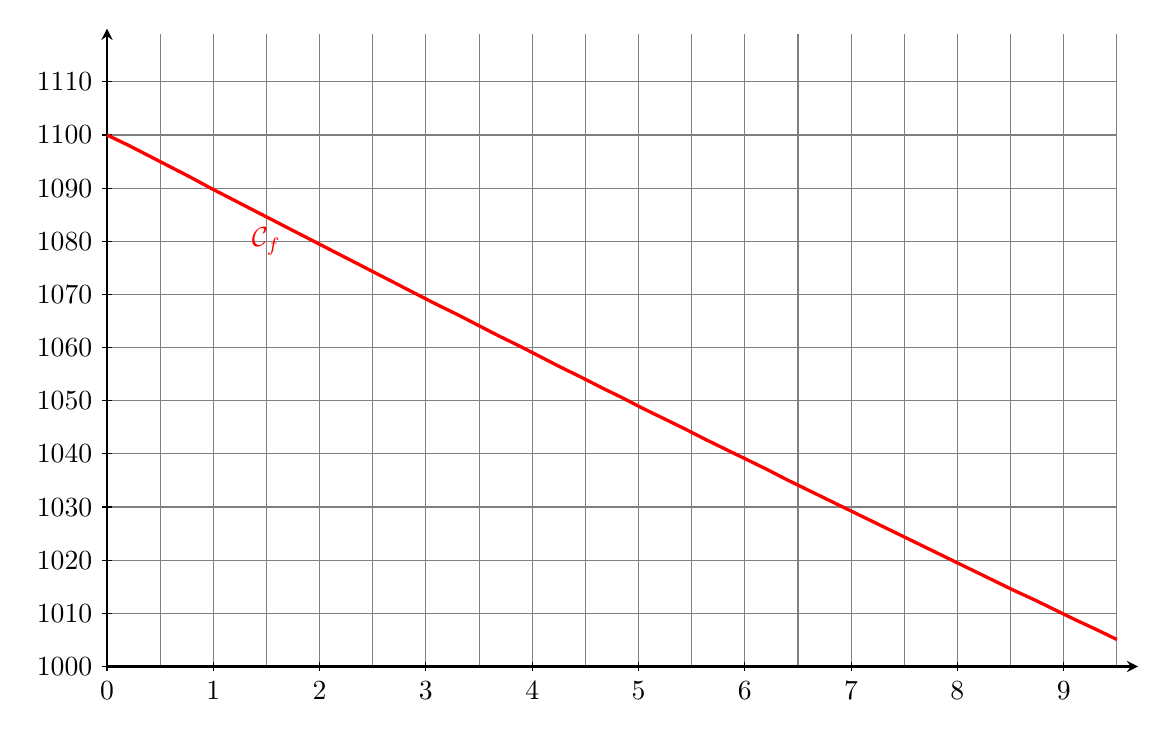
\begin{tikzpicture}[x=15mm, y=0.75mm,>=stealth,scale=0.9]
			\draw[xstep=0.5,ystep=10,gray,thin] (0,1000) grid (9.5,1119);
			\draw[->,line width=0.8pt] (0,1000) -- (0,1120);
			\draw[->,line width=0.8pt] (0,1000) -- (9.7,1000);
			\foreach \x in {0,1,2,3,4,5,6,7,8,9}
				\draw[shift={(\x,1000)}] (0,2pt) -- (0,-2pt) node[below] {\np{\x}};
			\foreach \y in {1000,1010,...,1110}
				\draw (2pt,\y) -- (-2pt,\y) node[left] {\np{\y}};
			\draw[red, line width=1.2pt] plot[domain=0:9.5,samples=50] (\x,{(1050*exp(-0.01*\x)+50)});
			\node[red] at (1.5,1080) {$\mathcal{C}_f$};
		\end{tikzpicture}
	\end{center}

		Lire, avec la précision permise par le graphique, l'année à partir de laquelle le niveau du lac sera insuffisant pour produire de l'énergie hydroélectrique.
	\end{enumerate}
